\documentclass{article}
\usepackage[utf8]{inputenc}

\title{Accessible Indoor Localisation for Android}
\author{Shubham Kapoor (014601220), \\Sebastian Hojas (014570704)}
\date{January 2016}

\usepackage{natbib}
\usepackage{graphicx}
\usepackage{listings}
\usepackage{minted}

\begin{document}

\begin{figure}
    \centering
    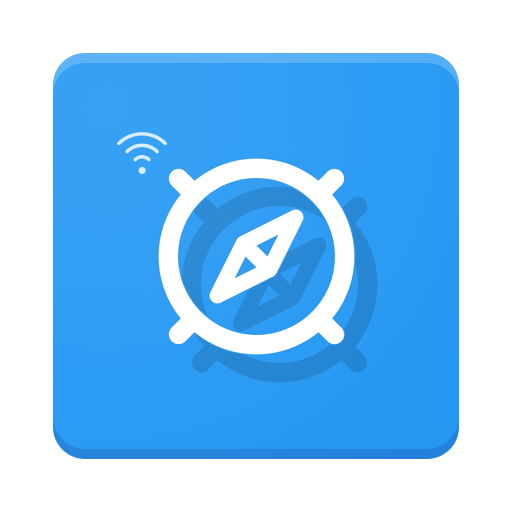
\includegraphics[width=0.3\textwidth]{icon}
    \label{fig:icon}
\end{figure}

\maketitle

\section{Introduction}
Locating ourselves has been a curious task for mankind for long. With the dawn of today's digital era various new wireless positioning techniques, such GPS, GLONASS, E-CID, OTDOA etc., were developed. These techniques provided overwhelming accuracy with a limitation: None of them worked accurately indoors and needed "clear" sky view for attending there promised accuracy. Moreover complex and diverse indoor environments make tracking indoor a tedious task. However increasing popularity of commercialized location-based advertising, indoor logistics, analytics etc. motivated industry to work on unexplored area of indoor localization. Various new techniques were devised for same ranging from magnetic to Wi-Fi positioning.

We developed a handy mobile Android application called \textit{Localiser}, which uses Wi-Fi positioning technique at its heart and calculates the devices's position in an indoor location with an accuracy of 5 meters. This application further gives the user details of point of interests near his/her location, such as nearby class rooms. Our app has implemented all native Android accessibility features, which would allow a visually impaired person to still use our app fluently and orient through campus.

\section{Features}

Some of the features of our application we want to highlight are:

\subsection{Show current Location} 

The application automatically shows the current location and updates it. Additionally, the user can use the button on the top right corner to center the current location on the map. The map will automatically change the displayed floor if the location changes.
The user can scroll and zoom the app to get a better overview.

\subsection{Nearby points of interest} 

This button is located next to current location button. Pressing this button displays nearby landmarks relative to current position of the user on the map. In our current version of our application we have defined around 100 classrooms and a couple of emergency exits (as seen in figure \ref{fig:location}), but this can be easily extended with more information about the building. 

\begin{figure}
    \centering
    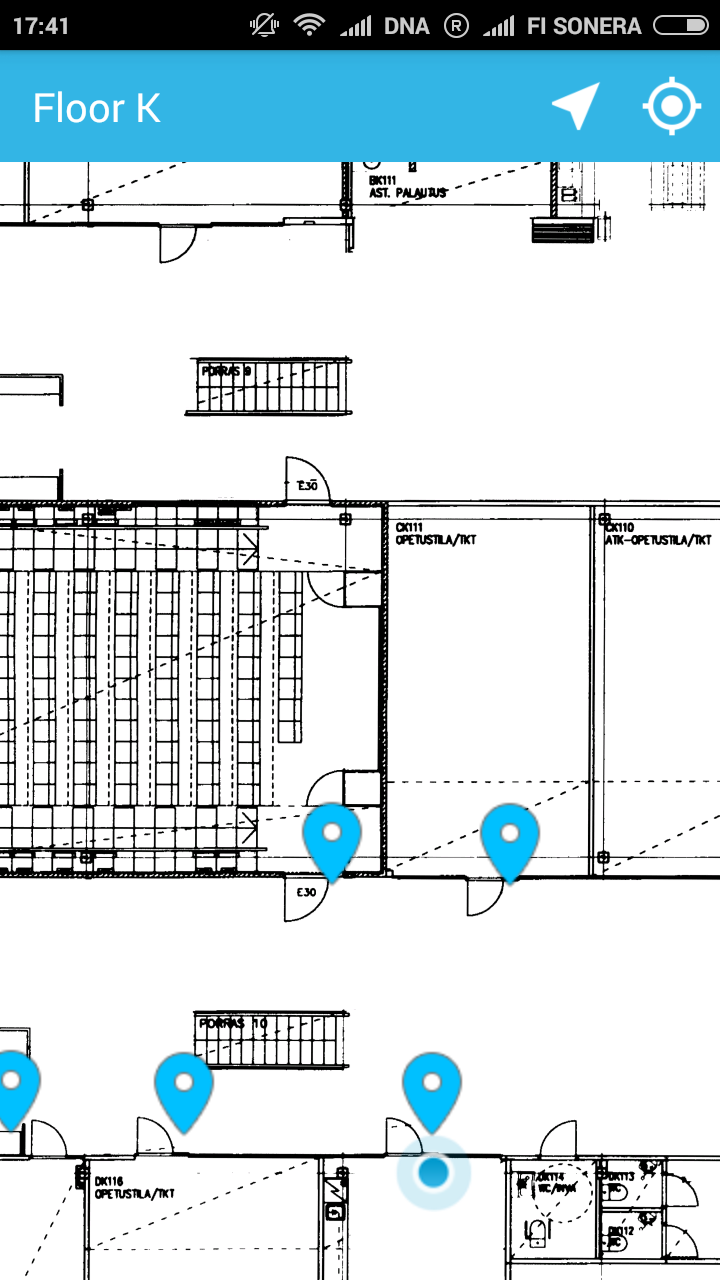
\includegraphics[width=0.5\textwidth]{Location}
    \caption{Screenshot of the application showing the current location and closest classroms nearby.}
    \label{fig:location}
\end{figure}

\subsection{Vertical position of user} 

The title of the current application displays the current floor number.

\subsection{Details of landmarks} 

If a user presses one of the displayed nearby landmarks, the user gets information about the landmark, as illustrated in figure \ref{fig:roominfo}. This includes its name and distance from the user. The user can then access the web-page of the defined landmark by clicking the information symbol which is at lower right corner of screen, as shown in figure \ref{fig:roominfo2}. Not all landmarks currently have a web-page associated with them. Hence the information symbol does only appear for classrooms that have a site on the website of the University of Helsinki.

\begin{figure}
    \centering
    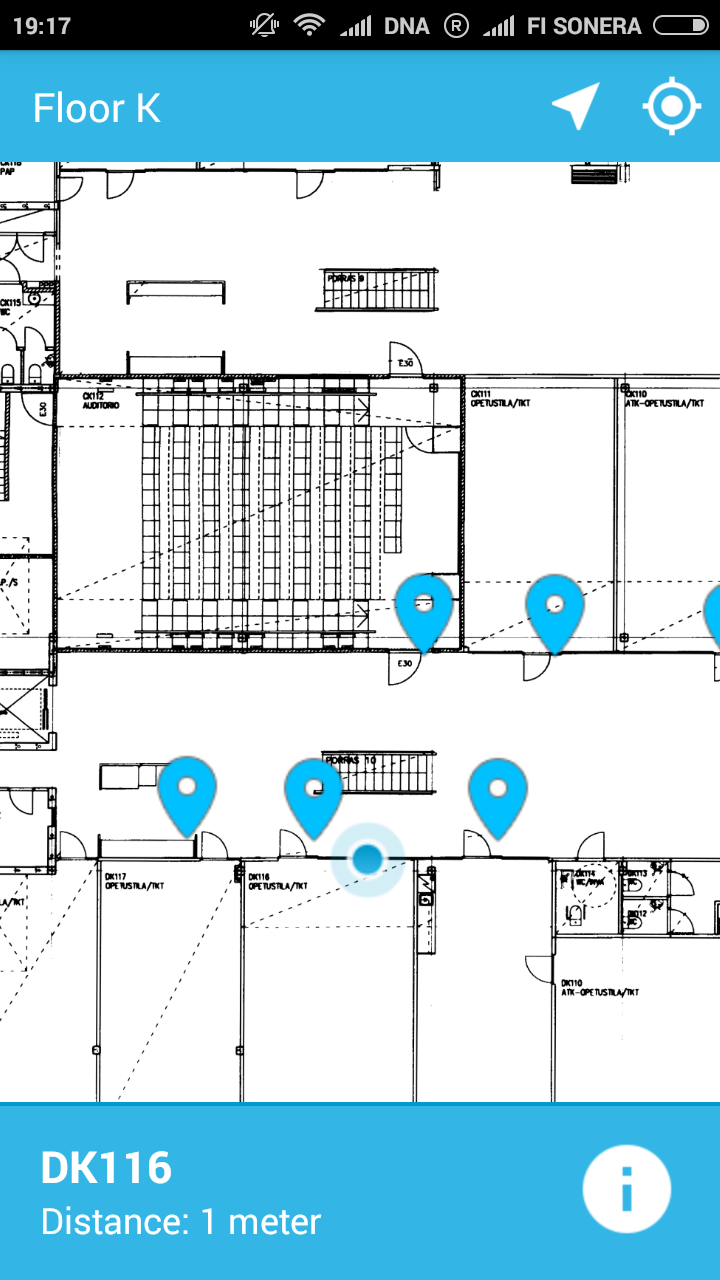
\includegraphics[width=0.5\textwidth]{Placeinfo}
    \caption{After a user tapped on a point of interest it shows its name and the distance to the user.}
    \label{fig:roominfo}
\end{figure}

\begin{figure}
    \centering
    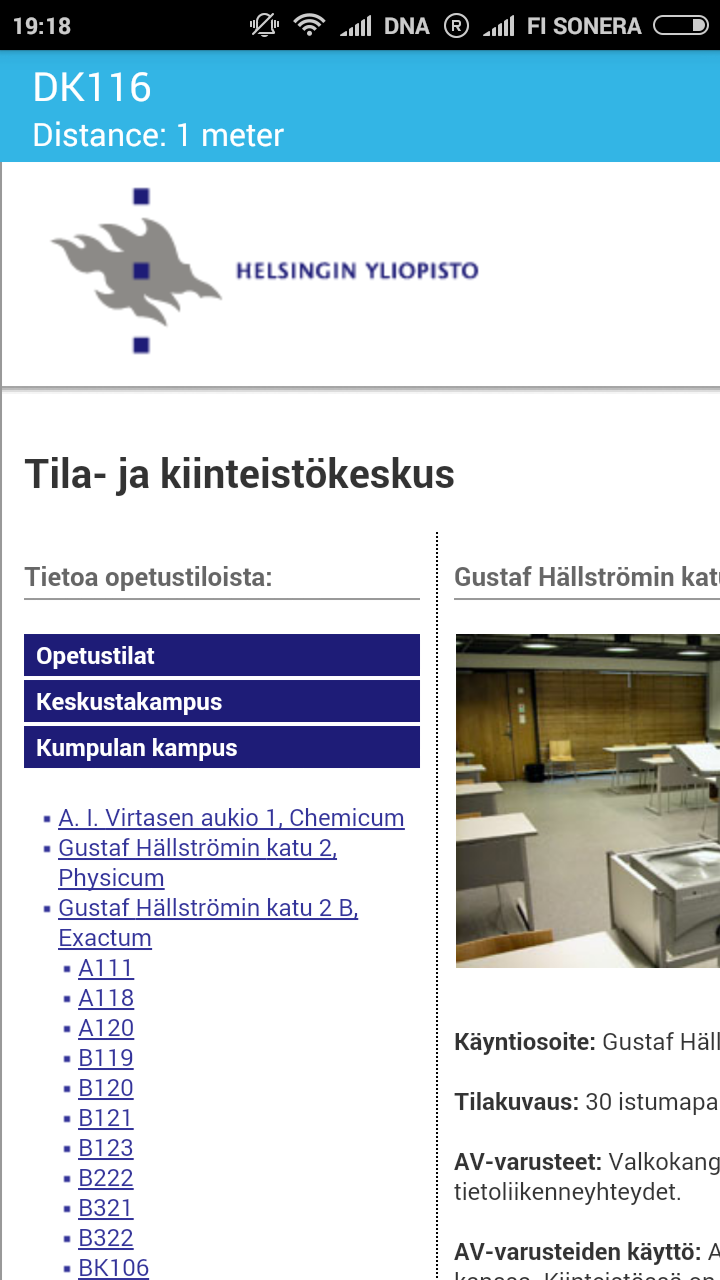
\includegraphics[width=0.5\textwidth]{Website}
    \caption{Some rooms link to the website of the University of Helsinki to show further information. This website includes information about the room size, its accessibility characteristics and contact information.}
    \label{fig:roominfo2}
\end{figure}

\subsection{Accessibility for visually impaired users} 

We have implemented native Android accessibility features that allow users who need assistance to use the application. We have successfully tested the application while being blindsided in accessibility mode Talk-back. We have made the following design decisions:

\begin{itemize}
    \item Every button and action has a content description that will be used by the Android Talk-back feature.
    \item This also includes all elements on the map. The current location will always be in the middle of the phone screen. If the users slides with his/her finger over the screen, nearby locations will be marked by vibrational and audio feedback as defined by the accessibility best-practise by Google. This also includes the distance in meters to the point of interest.
\end{itemize}

For further development we would suggest to use sensor data from the device's compass to be able to give the user information about the relative direction of the point of locations around the device.

\section{Algorithm}

The algorithm is the heart of the application that predicts the user's location with a probability $p$ for a given fingerprint. This algorithm is logically split into two parts:

\begin{itemize}
  \item \textbf{Fingerprint comparison (comparator)}: The comparator takes two fingerprints, compares them and calculates the similarity. We have observed that is the same problem class as string similarity calculation. Thus, we mainly implemented variations of known string comparison algorithms.
  \item \textbf{Location calculation}: Knowing the similarity of all fingerprints in the database to the reference scan, it is now easy to calculate the location. This calculation can be a simple closest match or an elaborate probability calculation.
\end{itemize}

\subsection{Fingerprint comparison}

We have implemented two different comparators:

\begin{itemize}
  \item \textbf{Intersection matching}: Considers only the intersection of two fingerprints and calculates the similarity of observed signal strengths of both data sets. This is a simple approach with a higher error rate because it favours fingerprints with small subsets and matching signal strength.
  \item \textbf{Cosine matching:} The cosine comparator considers the whole subset and therefore delivers more accurate results. It calculates the cosine similarity between the two fingerprints. We use this comparator by default.
\end{itemize}

\subsection{Location calculation}

\begin{itemize}
    \item \textbf{Nearest Neighbor}: The algorithm matches the fingerprint with the highest similarity and takes its location.
    \item \textbf{k-Nearest Neighbors}: The algorithm matches the $k$ nearest neighbors and calculates the coordinates based on the weighted location of all fingerprints.
    \item \textbf{Average}: For localisation, we wanted to implement a high/low pass filter that uses the median to improve accuracy. For simplicity, we implemented an average algorithm that takes $n$ measurements, calculates $n$ locations with the k-nearest-neighbors-algorithm and takes the average. This reduces average jumps (especially to avoid sudden changes of the $Z$ value). The high fingerprinting frequency of our test device allowed us to still update the location approximately every three seconds, which is enough for our use case.
\end{itemize}

The next step would be to extend the average algorithm and create a more complex probability model (i.e. a Kalman filter) which also considers probability of changes in time and input from the motion sensors (gyroscope, compass and accelerometer). This way, we believe, we could increase the accuracy tremendously.

\section{Database}

The matching algorithm uses a data set of 1592 fingerprints. We created an individual Android application for the collection of fingerprints. It followed this simple workflow:

\begin{enumerate}
    \item Define a path with $n$ steps and confirm.
    \item The application will then ask the user to walk through the path, stopping at every defined step.
    \item While the user walks, the application takes as many fingerprints as possible and calculates an approximated location based on the assumption of linear walking speed between each stops, as shown in figure \ref{fig:collecting}.
    \item At the end of the path, the user can save the appended database file on the SD card. The new dataset is then ready to be manually downloaded from the phone.
\end{enumerate}

The application can be started by launching \textit{CollectFingerprintsActivity} and needs \textit{android.permission.WRITE\_EXTERNAL\_STORAGE} which is temporarily disabled for the production. We chose to create an Android application to enable the collection of fingerprints with a mobile device.

\begin{figure}
    \centering
    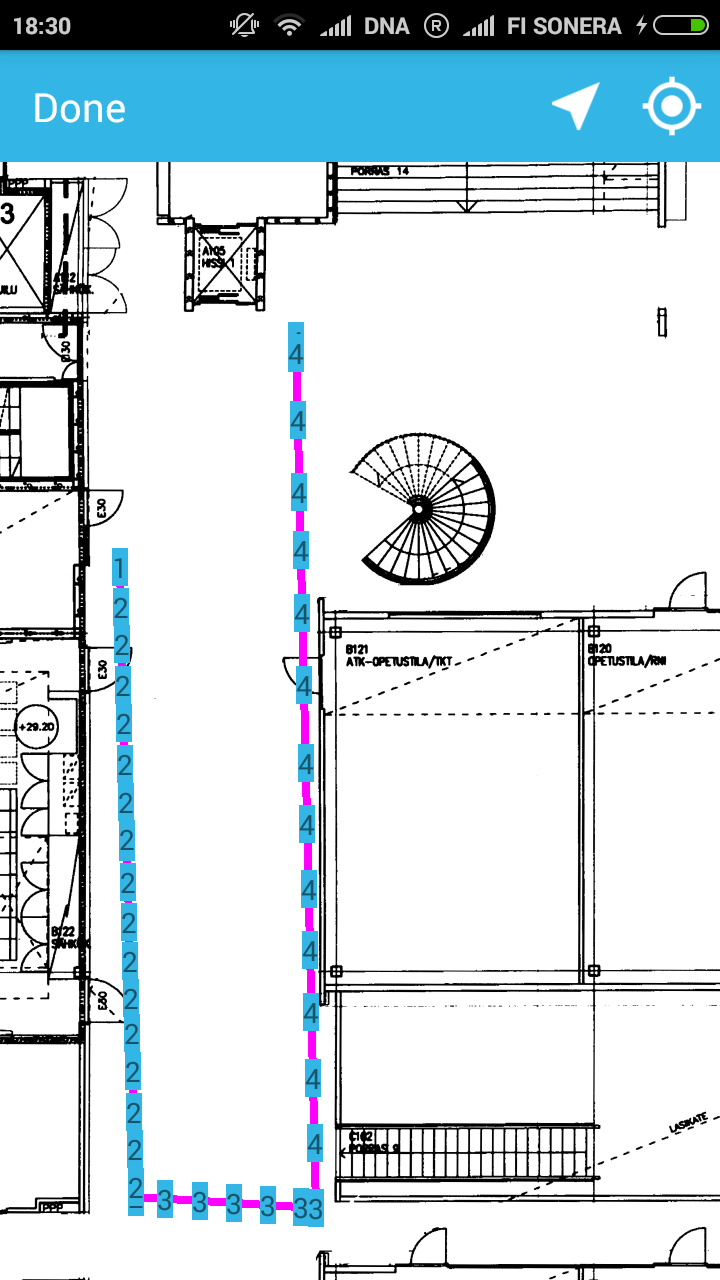
\includegraphics[width=0.5\textwidth]{Fingerprints}
    \caption{Example how we used our Collector application to massively collect fingerprints}
    \label{fig:collecting}
\end{figure}

% TODO show demo pictures of walker

\section{Software Architecture}

The Android GUI activities use the \textit{LocaliserController} to register for location events. When initiating the controller, an algorithm can be chosen. Every algorithm can use a different comparator, that defines how fingerprints are being compared to each other. This allows the activity to easily choose the used algorithm and its comparator.\\

Usage of a controller with the \textit{k-nearest-neighbors} algorithm with the \textit{Cosine} comparator would be the following:

  \begin{minted}[%
  breaklines]{python}

AbstractLocaliserAlgorithm algo = new kNearestNeighborsAlgorithm(new CosineComparator());

try{
    LocaliserController testController = new LocaliserController(algo, context);
    testController.registerForLocationUpdates(this);
}
catch(LocaliserController.NoWIFIException err)
{
    // TODO error handling: WIFI was disabled
}
catch(IOException err)
{
    // TODO error handling: Could not read database
}
\end{minted}

This dynamic architecture allowed us to change location algorithms and comparators easily and even test different combination simultaneously. 

\section{Testing}

We have developed our application for the following platforms. We would be available for the demonstration of the application on our tested device.

\subsection{Platform}

We have successfully tested our application on a \textit{Xiaomi Redmi 1S device}. The device has a 1.6GHz Quad-core Qualcomm Snapdragon 400 processor with Cortex-A7 core. The device has 1 GB of RAM and 8 GB of FLASH internal memory. This device supports standard Wi-Fi 802.11 b/g/n. Our device runs on android Kitkat with API level 19. While we developed our application for API level 14 and above, we have not been able to test our application on different Android device and different API levels.

\subsection{Accuracy} 

The current version of our application gave us an accuracy of about 5 meters with the above mentioned test device. We have covered the area in Exactum as defined for the first assignment, without the locked computer lab. We also tested in-room localisation in the 24/7 computer-lab and have been very satisfied with the accuracy in closed and open spaces.

\end{document}

